\documentclass[11pt, oneside]{article}   	% use "amsart" instead of "article" for AMSLaTeX format
\usepackage{geometry}                		% See geometry.pdf to learn the layout options. There are lots.
\geometry{a4paper}                   		% ... or a4paper or a5paper or ... 
%\geometry{landscape}                		% Activate for rotated page geometry
%\usepackage[parfill]{parskip}    		% Activate to begin paragraphs with an empty line rather than an indent
\usepackage{graphicx}				% Use pdf, png, jpg, or eps§ with pdflatex; use eps in DVI mode
								% TeX will automatically convert eps --> pdf in pdflatex		
\usepackage{amssymb}
\usepackage{amsmath}
\usepackage{authblk}
\usepackage[hyphens]{url}

\usepackage{url}
\usepackage{hyperref} 

\usepackage{titlesec}

\usepackage{caption}

\usepackage{float}


\title{Ecosystem Services Management: From Alarm to Action}
\author{Aidan T. Parkinson; Andreea M. Benu}

\date{\today}							% Activate to display a given date or no date

\begin{document}
\maketitle
\begin{center}
\href{mailto:enquiries@aidantparkinson.com}{enquiries@aidantparkinson.com}
\end{center}

\section{Abstract}


\section{Introduction}

We live in an age where global crises, such as climate change, biodiversity loss, and geopolitical instability overlap and compete for attention.
Yet our tools for cooperation are often inadequate.
Such unrest raises a deeper question: how societies coordinate fairly when nation-states alone cannot manage the global commons?\\

For centuries, thinkers from Hobbes to Rawls have debated how communities balance self-interest with duty to the wider world.
Their ideas provide language for rethinking today's ecological governance.
John Rawls, for example, argued in the The Law of Peoples that \emph{"Peoples have a duty to assist other Peoples living under unfavourable conditions that prevent their having a just or decent political and social regime."}~\cite{jr2}.
But in truth, everyone today lives under some form of unfavourable conditions.
This means all of us share a duty to assist the systems that make life possible: biodiversity; basic utilities; reasonable shelter; security.
Is it realistic to imagine an entirely reasonable society unaffected by the imperfect Realpolitik of nation-states?\\

Philosophers describe the \emph{"State of Nature"} as life without shared rules: sometimes pictured as cooperative~\cite{jl1}~\cite{rn1}, other times as chaotic and conflict-ridden~\cite{th1}.
If our global order resembles such a State, what responsibilities do we still owe each other?
Should they fall predominantly to nation-states, to individuals, or to an intergovernmental organisation?
What can a reasonable person do for the common good?
How might such efforts be organised into a fairer society?
Neither the reasonable society Rawls envisions, nor the sovereign authority Hobbes demands, seem wholly adequate for today's ecological and political realities.
We evidently live in a hybrid system, too imperfect for a reasonable utopia and too plural for absolute authority.\\

This tension suggests ordinary people and institutions alike share a responsibility.
One not grounded in perfection, but in doing the \emph{"the best we can do."}
Our argument is that this \emph{"best we can do society"} provides the more complete form of social contract that Rawls anticipated, but did not fully realise.
As a result, this paper argues for a society that we call a \emph{"Commonwealth of Peoples"}.
Such a society of individuals does not promise utopia, but more practically, the best that can be done.
Here, all society have a duty of minimal service in common relating to an ecosystem performance observation which is equal to our novel \emph{"Commonwealth Cost of Carbon"} definition.
Where Rawls imagines a perfectly reasonable society of cooperating cooperating Peoples, the Commonwealth of Peoples sets out to endure deep rooted philisophical pluralism and stubborn disagreement on pivotal global questions.
Such a framework exhibits the resilience needed for taking meaningful action in the interest of the commons, constrained by the realpolitik of nation-states.
We find the Commonwealth of Peoples a more workable social contract: one in which imperfect actors can still coordinate fairly by balancing their duties to one another with impacts on the wider ecosystem.
It acts to renew our focus on demand-side assurance and advisory for private legal entities, whilst maintaining global perspective.
Over time, the Commonwealth of Peoples has potential to scale universally across all end-use services.\\

At this point of departure, this research moves from an exploration of theory to breaking entirely new ground.
To move from principal to practice, the remainder of this paper discusses the societies strategic planning whilst considering action.
Such an exercise is limited to the authors combined experience, but works to illustrate our shared vision for development.
A newly formulated \emph{"Service Rating"} is proposed to support classification of end-use services, with an essential dependency on the Commonwealth Cost of Carbon.
This is included as a key driver within a prospective scenario planning exercise that define expectations for a new ecosystem services performance marketing application.
We conclude with a reflective evaluation of this initatives achievements and present limitations.\\


\section{Ecosystem Performance Observation}

Can a society realistically be free of the Realpolitik and territorial disputes that influence the politics of nation-states?
We would argue that everyone themselves subject to nation-states and must serve at least minimal compliance.
It is common for the most reasonable societies to find themselves in situations where they must comply with a political decision that they don't agree with.
Such occurrences lead to ecosystem externalities, also known as social costs, that need internalising into decision-making for enduring action~\cite{rc1}.
This exercise, observing ecosystem performance, then is considered a necessary additional instrument for any model \emph{"best we can do"} social contract.
So, how could such observations be made?\\

When examining carbon-based life, such as humans, it is natural to take an interest in their activities and bi-products when investigating performance.
Certain items of waste, such as consumer goods packaging and water quality, might be tended well by the authorities of territories.
However, when all accounted for, greenhouse gas emissions are a by-product of any human agreement anywhere.
Such anthropogenic emissions are vented to a common ecosystem, for which many might expect an equitable share.
The state of our common ecosystem on planet Earth is maintained by carbon sinks that absorb the greenhouse gas emissions of anthropogenic activities.
"Enabling Assets" is a term we use to account for the roles of institutions, knowledge, time and networks in production~\cite{pd3}.
These assets have a natural relationship with carbon sinks, that can be defined as software.
The positioning and use of Enabling Assets are a pivotal consideration when seeking to understand human impacts on our shared ecosystem.
It is with this understanding that we believe it is reasonable to assert that nobody can entirely delegate responsibility for energy management.
Energy management is a deep rooted science that involves every decision and agreement anyone makes, including the most senior of occupations.
An alternative goal of economic growth appears more relevant to the successful servicing of national debts.
Could the state of our carbon sinks be a more interesting measure of overall ecosystem performance?\\

\subsection{Utilitarian Perspective}

Calculation of a Social Cost of Carbon to measure the state of the ecosystem has proven to be highly rewarding for those taking utilitarian perspectives, prescribing happiness as a whole as the ultimate end to action ~\cite{hs1}.
The resources consumed in satisfying human needs require economic considerations to efficiently manage personal well-being.
Normative economists often regard only individual circumstance, or level of  welfare, in a state of affairs as important.
This is known as the neutrality assumption~\cite{pd2}.
Arrow, May and Sen assert that this position of neutrality is effectively an avocation of anonymity with respect to social states, which is a requirement that human beings be treated equally~\cite{ka1}~\cite{km1}~\cite{as2}.
Waldron defines the notion of social welfare, an aggregate of individual welfare, as being goal-based~\cite{jw2}.
Dworkin states that a goal can be considered a non-individuated political aim~\cite{rd1}.\\

Early contributions to address this research question were awarded the Nobel Prize~\cite{np1} and life peerages in the House of Lords~\cite{g1}.
These notable precedents prescribe aggregate or social welfare as a goal for social benefit.
Aggregate welfare is not evenly distributed amongst the worlds population.
Therefore, pure reinforcement of aggregate welfare is largely in the interest of a few wealthy people.
This approach typically employs Frank Ramsey's Mathematical Theory of Saving as a decision-making tool.
The process involves creating complex integrated assessment models of humanities social and environmental systems that apply gross assumptions of Earth's development.
Mechanisms that determine the state of the world are identified and the consequences of alternative policies charted so that consequences can be valued.
Welfare surpluses are then estimated for policy options, by making projections of differences from the \emph{status quo} 100's of years into the future.
Valuation of these surpluses involves setting a global social discount rate and this requires a set of personal assumptions.
As a result, these economists offer estimates of a \emph{"social cost of carbon"}~\cite{pd2}.
A summary of the underlying decision-making criteria is shown follows~\cite{fr1}:\\

\begin{equation}
V_t = \sum_t^\infty \beta^{(\tau - t)} \cdot U (C_\tau)
\qquad \text{for }
\qquad t \geq 0
\end{equation}

Where,
\begin{equation}
\beta = \frac{1}{(1+\mu)}
\end{equation}

Where, $V_t$ is \emph{a generations welfare}, $\beta$ is the \emph{discount factor}, $U$ is \emph{welfare}, $C_\tau$ is \emph{consumption during time-step}, $t$ is \emph{time} and $\mu$ the \emph{social discount-rate}.\\

\begin{equation}
\mu = \sigma \cdot g + \delta
\end{equation}

Where, $\sigma$ is the \emph{marginal utility of consumption} and the difference in the utility one would gain from a unit of consumption by those of low and high incomes, $g$ is the \emph{long-term growth rate} in consumption, $\delta$ is the \emph{pure rate of time preference} and our impatience to consume in fear of extinction.\\

\begin{equation}
S = \frac{\mu-\delta}{\sigma \cdot \mu}
\end{equation}

Where, $S$ is the \emph{savings rate} and the proportion of output that should be invested.\\

This complex process results in considerable disagreement amongst social cost of carbon estimates for a historic time period using this method.
The assumptions for a global social discount rate used for three early contributions are provided in Table~\ref{Social contributions table}.
The global social discount rate for these three contributions ($\mu$) is similar.
However Cline is outlying in estimation of the difference in utility the wealthy gain from a unit of consumption compared to the poor ($\sigma$).
None of the three contributions agree on a long-term global growth rate ($g$).
When considering impatience to consume in fear of extinction ($\delta$) it is Nordhaus that appears outlying.
This yields very different values for the amount of surplus to be saved relative to that consumed amongst the three contributions ($S$).
Clearly the worlds envisioned by just these three notable precedents are really quite different in nature and perhaps the reality is that the ethical positions of these contributors are in competition.
Anyones candidacy of representing the \emph{"ideal observer"} to follow here is very likely to be considered grandiose and illegitimate.
For most, the setting of these assumptions is of private preference only.
Nevertheless, such economists and many followers since have contributed social costs of carbon in the interest of the commons.
Some of these assessments have had privilaged access to the development plans sitting US administrations, as perhaps leading candidates for the commons ideal observer.
However, in reality, nobody has the power to set a social discount rate in this way for all.\\

\begin{table}[H]
\caption{Notable Precedents: Assumptions in Social Discounting}
\begin{center}
\begin{tabular}{| l | c | c | c | c | c |}
\hline
Contribution&$\mu$&$\sigma$&$g$&$\delta$&$S$\\
\hline
Cline, 1992~\cite{wc1}&0.05&1.5&0.033&0&0.67 \\
Nordhaus, 1994~\cite{wn1}&0.05&1&0.02&0.03&0.4 \\
Stern, 2006~\cite{ns1}&0.05&1&0.049&0.001&0.98 \\
\hline
\end{tabular}
\end{center}
\label{Social contributions table}
\end{table}

Figure~\ref{USA SCC figure} is a graphical representation of Social Cost of Carbon estimates by the Interagency Working Group on Social Cost of Carbon, United States Government.
This meta-analysis considers the results of three pioneer integrated assessment models developed in the 1990's.
These are the DICE, PAGE and FUND models~\cite{wn1}~\cite{ch1}~\cite{rsjt1}.
The modelling simulations considered by this study returned a Social Cost of Carbon anywhere between $<$2007\$0tC\textsuperscript{-1} to a 95th percentile of 2007\$128tC\textsuperscript{-1} with $\mu$ set at 0.03~\cite{iwg1}.
Based upon these results for a Social Cost of Carbon, it is clear that utilitarians would find it difficult to significantly alter their actions and agree on options to be taken. \\

\begin{figure}[H]
\centering
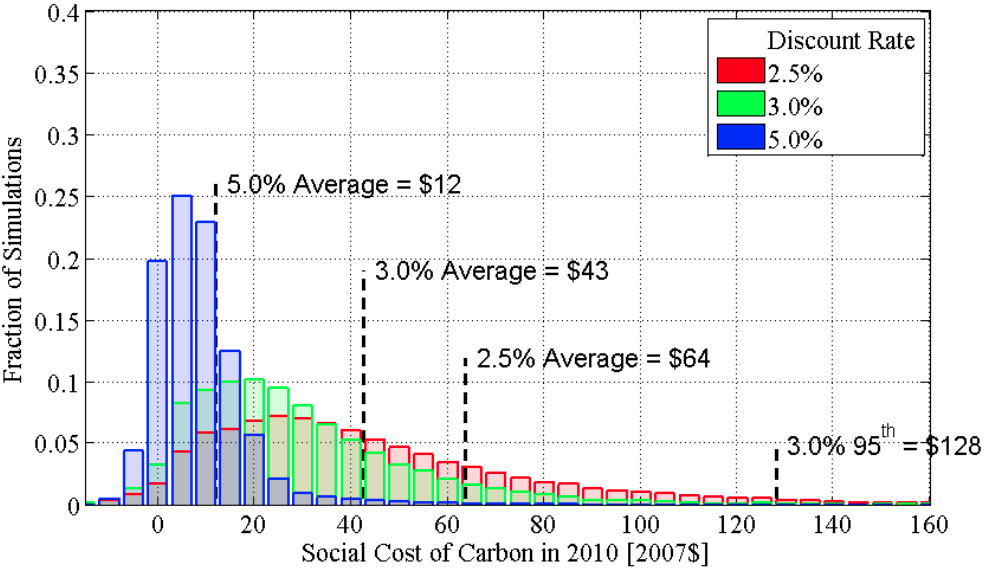
\includegraphics[width=1\textwidth]{scc}
\caption{Social Cost of Carbon in 2010 (in 2007 dollars per metric ton)}
\label{USA SCC figure}
\end{figure}

\begin{quote}
"Here there are a number of possibilities. A collective decision may determine the rate of saving while the direction of investment is left largely to individual firms competing for funds. In both a Private Property as well as in a socialist society great concern may be expressed for preventing irreversible damages and for husbanding natural resources and preserving the environment. But again either one may do rather badly."~\cite{jr1}
\end{quote}

Collective saving for the future has many aspects of a public good, though under conditions of arising problems of isolation and assurance~\cite{as1}~\cite{ms1}.
Even among welfare economists, some reject applying pure time preference so that one allows the living to take advantage of their position in time to favour their own interests~\cite{hs1}~\cite{fr1}.
Such examples ignore the possibility for the living to wrong their predecessors or descendants.
Dasgupta argues that it is one thing to urge that an imperfect economy should be improved, quite another to pretend that the imperfect economies we inhabit are Utopia in the way these contributions suggest.
Those who follow the principles of the social contract when taking action would probably find these methods have little relevance to their sense of justice.
These contributions also do not consider the possibility for states of affairs to deliver imperfect procedural justice leading to noncompliance.
Libertarian's might argue that such collective action would lead to violations of individual rights to even a slight extent and therefore should be rejected~\cite{rn1}.
Advocates of the free-market may criticise such methodologies that involve seeking prosperity through centralised long-term coercive planning, rather than appropriate regulation that allows local agents to adjust their activities according to the present situation~\cite{fh1}.
There is indeed nothing sacrosanct about the public decision concerning the level of savings and its bias with respect to time preference deserves no special respect~\cite{jr1}.
Therefore, an alternative proposition is sought.\\

\subsection{Hobbesian Perspective}

An alternative perspective is to use the principles of the social contract to estimate a \emph{"Commonwealth Cost of Carbon"} for decision-making.
Here, one cannot rely on the assumption that the ideals of liberal democracy or social welfare are necessarily shared by all those affected.
However, one might assume acknowledgement between parties of an ecosystem represented by a Hobbesian \emph{"State of Nature"} with allowances for political compromise and Realpolitik.\\

The problem is to use Hobbesian thought to value the cost of common ecosystem externalities.
Dasgupta asserts that this valuation need involve comparison of worlds with and without greenhouse gas emissions and stable currency~\cite{pd2}.\\

Ones understanding of the carbon cycle helps us determine that a world without greenhouse gas emissions is a world without life.
The Moon is an example of a world without a significant carbon cycle.
Carbon emissions appear an essential good that life cannot do without, deeply embedded in development.
What might be important here is not the quantity of greenhouse gas emissions, but the quality of greenhouse emissions.\\

The next task is to understand what a world would be like without stable currency.
Hobbes would suggest this be a war of \emph{all against all}, a world without submission to an absolute authority.
There is currently no common sovereign power over the entire ecosystem.
Hence, currency isn't entirely stable and territorial disputes do present themselves regularly.
To maintain confidence, citizens of well-ordered societies will normally want the rule of law maintained.
Although we might acknowledge that a common sense of justice is shared and that each wants to adhere to its arrangements, one might nevertheless lack full confidence in one another.
One might suspect that others are not doing their part, and so may be tempted not to do theirs.
The general awareness of these temptations may cause social systems to break down.
The role of a public interpretation of rules supported by collective sanctions is needed precisely to overcome this instability.
For this reason alone, coercive nation-states appear always necessary, even though in a well-ordered society sanctions may be slight and may never need be imposed.
Therefore, the penal machinery of nation-states becomes ones security to another and is entirely sacrificial~\cite{jr1}.\\

Therefore, to account for ones service to sustain a life worth living, one arrives at an ecosystem performance observation equivalent to a \emph{Commonwealth Cost of Carbon} for a given time-period:\\

\begin{equation}
	\frac{anthropogenic\; expenditure\; on\; enforcement}{anthropogenic\; greenhouse\; gas\; emissions}
\end{equation}\\

It is evident that this calculation method requires relatively straightforward maths, but the accounting is not trivial.
As a worked example, one has determined point estimates for the Commonwealth Cost of Carbon in Reporting Years 2000 to 2020.
Greenhouse gas emissions and gross domestic product of each nation-state were collected from the World Banks published World Development Indicators in 2024, consisting of 224 Reporting Nations out of 266 nation-states~\cite{wbank}.
Reported expenditures of nation-states on defense, public order and safety were collected from the International Monetary Fund Data Portal in 2024~\cite{imf}.
Here, it appears Reporting Nations account for ninety eight percent of total global expenditures.
Helpfully, the International Monetary Fund also reports Global gross domestic product.
Global greenhouse gas emissions were inferred for each Reporting Year by dividing Global gross domestic product by the sum of Reporting Nations gross domestic product, before multiplying this ratio by Reporting Nations greenhouse gas emissions.
Global enforcement expenditures were inferred for each Reporting Year by dividing Global gross domestic product by the sum of Reporting Nations gross domestic product, before multiplying the resulting ratio by the sum of Reporting Nations expenditures on defense, public order and safety.\\

A Commonwealth Cost of Carbon has been calculated for each Reporting Year, with the results presented in Figure~\ref{CCC figure}.
The figure appears to demonstrate a trend of degrading ecosystem performance over the Reporting Years.
Such insight appears to suggest the action to save greenhosue gas emissions have become more valuable.\\

\begin{figure}[H]
\centering
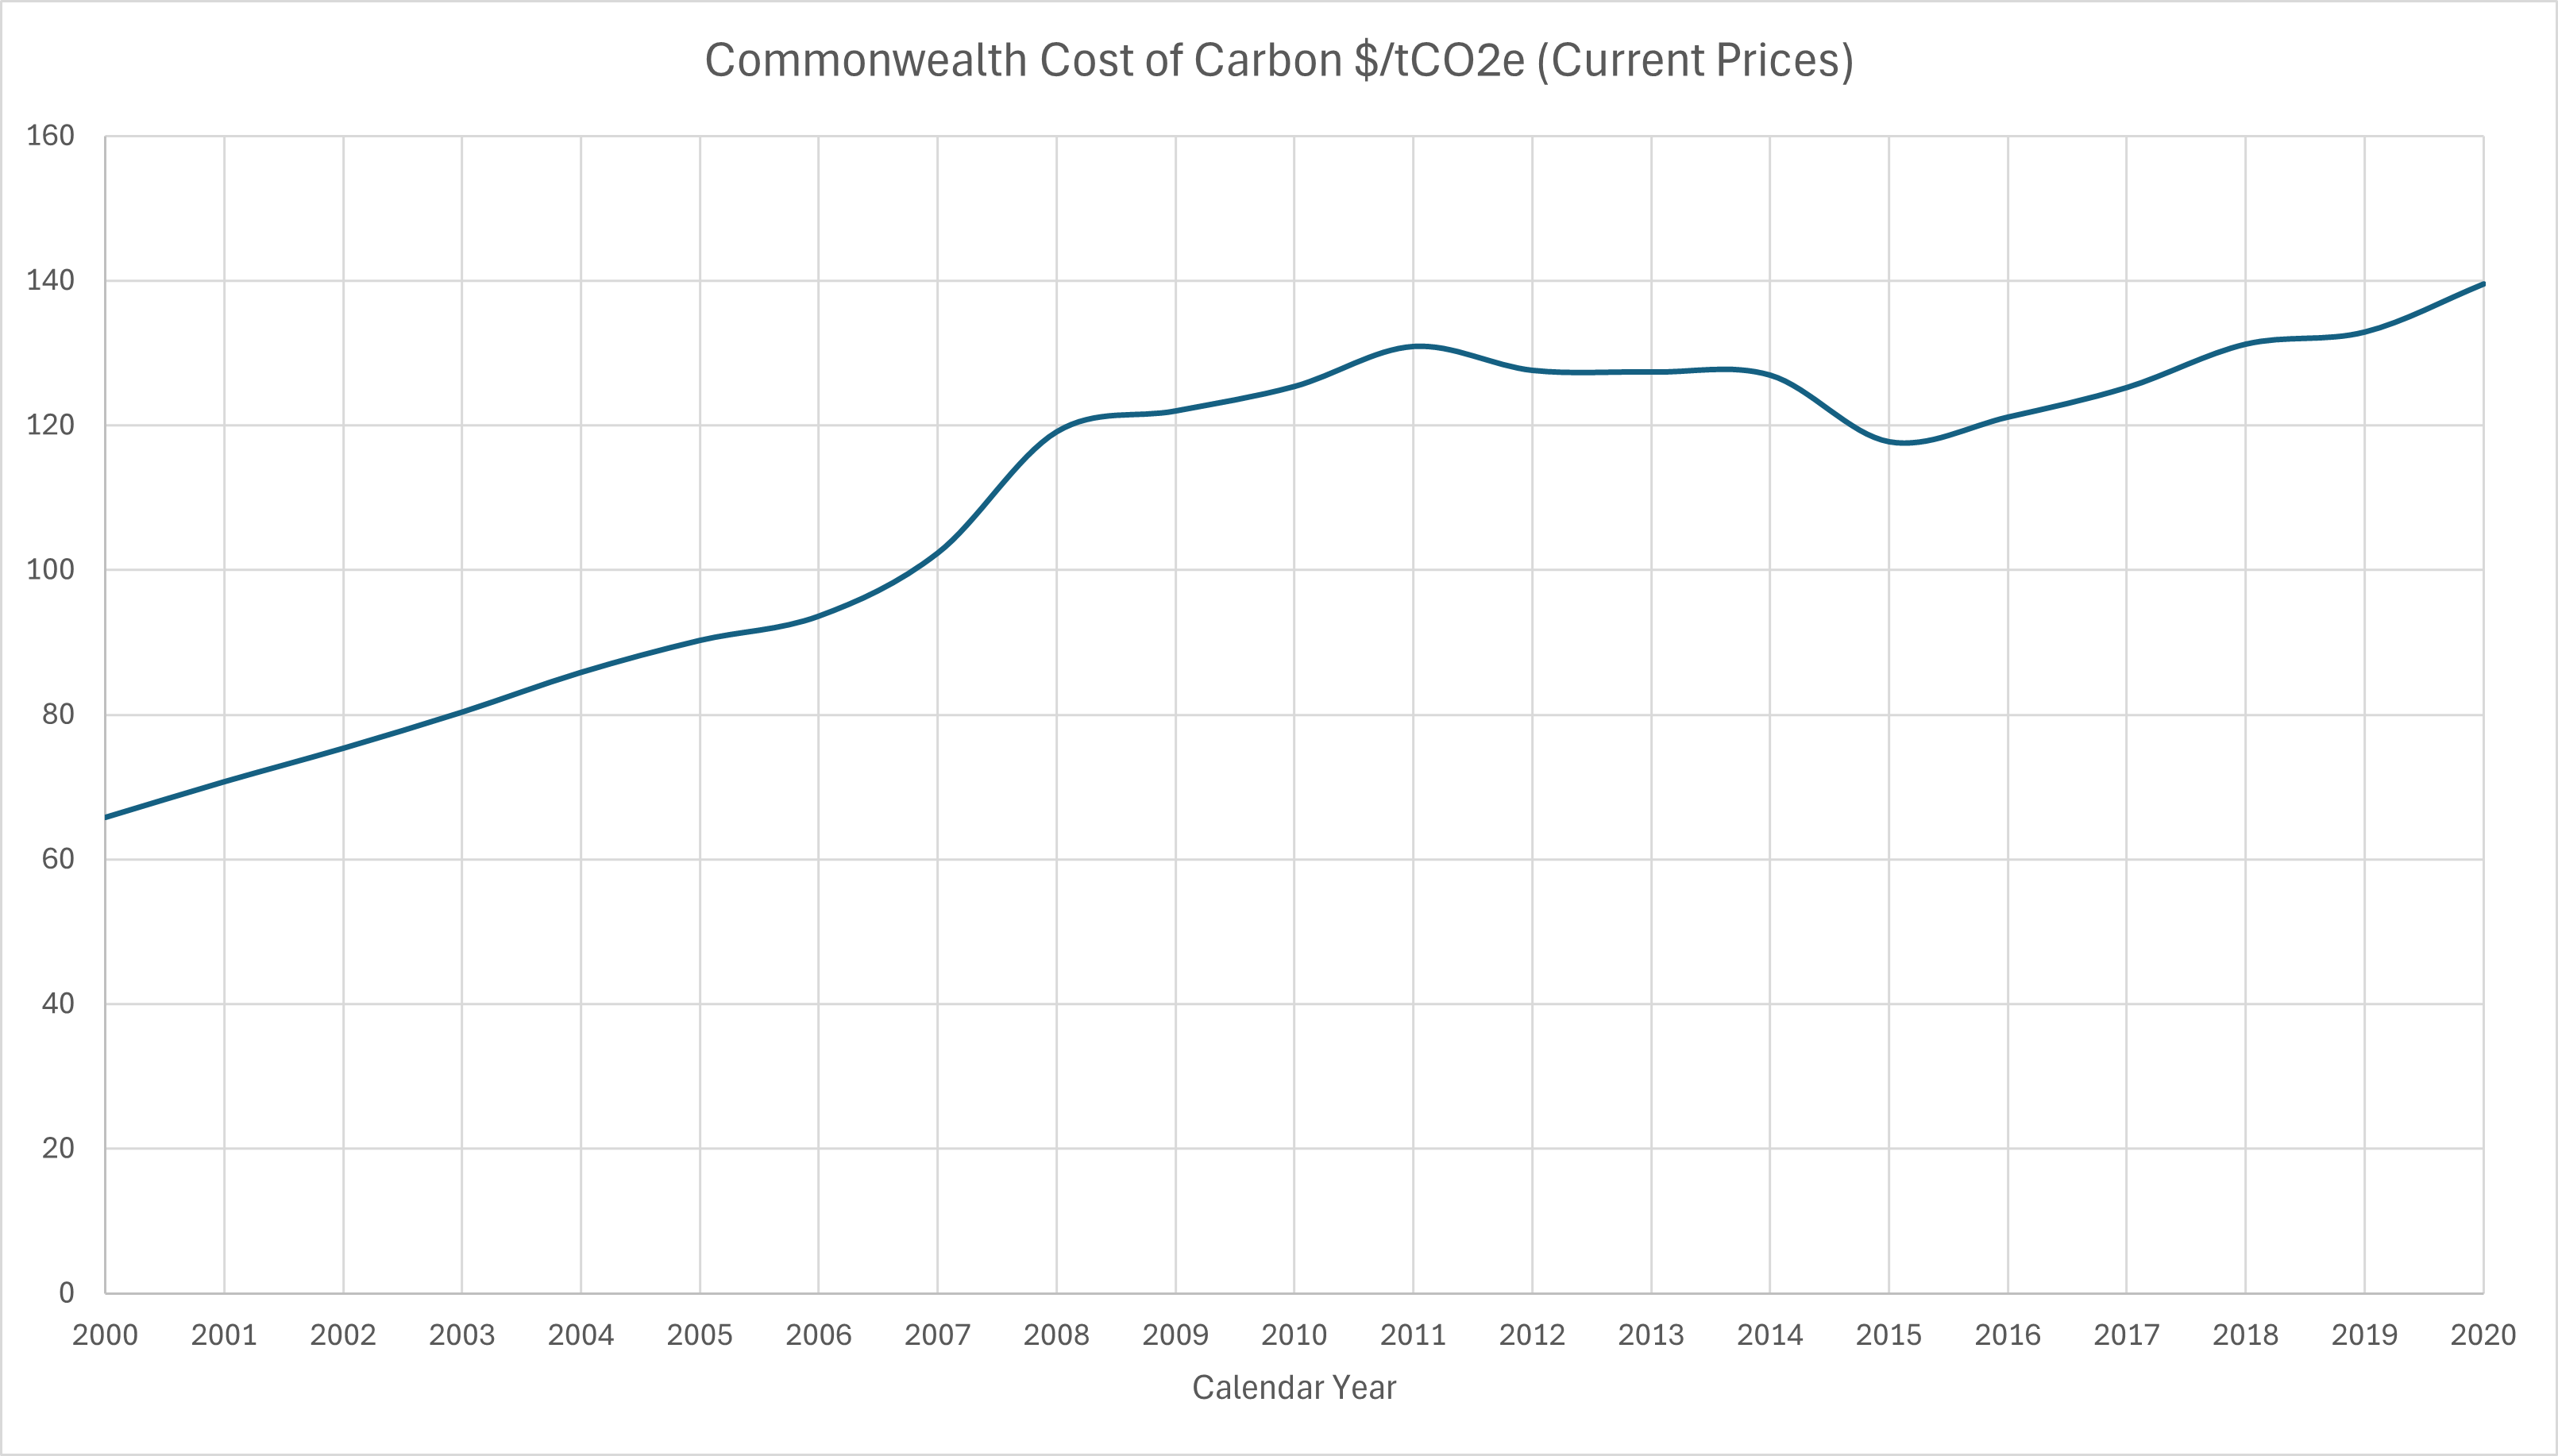
\includegraphics[width=1\textwidth]{ccc}
\caption{Commonwealth Cost of Carbon \$tCO2e (current prices)}
\label{CCC figure}
\end{figure}

\section{Strategic Planning}

This research has established a global ecosystem performance indicator applicable to ones entire history.
Such insights provide the opportunity to embed long-term strategy for sustainable action.
When applying the Commonwealth Cost of Carbon in addition to John Rawls Principles of a Society of Peoples, one arrives at an original constitution of a \emph{Commonwealth of Peoples}.
At this point the constitution of the Commonwealth of Peoples is considered comprehensive philisophical doctrine, both a stable and protected belief.
One is also mindful of the possibility that some may find spiritual connections with any indicator that measures a societies sacrifice to maintain the status quo.
The Commonwealth Cost of Carbon certainly appears an instrument that requires due respect.
Although, the Commonwealth of Peoples is established as an inter-networking or inter-faith foundation that offers nothing to necessarily worship in itself.\\

Our constitution is not enough to promote wider engagement and action.
It is our proposition that some sort of vision, hypothesis or prospect is needed for a shared understanding.
We recognise that small changes to the quality of services can have significant impacts on requirements for supply infrastructure.
Realising infrastucture savings could be a more fruitful activity than simply making radical changes to the quality of infrastructure provided.
Therefore, the management of service quality appears a strong candidate for action.
How can a Commonwealth Cost of Carbon be used to inform service performance marketing?\\

An exercise in strategic planning from our newly identified position was initiated.
Parkinson et al. outlines a useful taxonomy of methods for scenario planning, which may be used~\cite{atp1}.
An exercise of prospective scenario planning is a recognised methodology to explore qualitative possibilities for developing longer term plans.
Such techniques consider what could conceivably happen, rather than determining probable or preferred outcomes.\\

As this initiative was something of an outcast, we did not the opportunity to engage a wider group of peers.
It would have been preferrable at this stage to include a large workshop of experts within this exercise.
Therefore, ones scenario planning has been undertaken by the authors alone.\\

Initially, this research set out to establish two driving forces.
It is believed that one of these driving forces involved the magnitude of the service, represented by service cost.
One also determined that another driving force required a \emph{"Service Rating"} representative of the quality of service greenhouse gas emissions.
Such a Service Rating can be used to compare the performance of services on a consistent basis anywhere worldwide.
One applied the following equation to establish Service Rating for a consistent period of time, which is conceived as a simple cost-benefit ratio.\\

\begin{equation}
	\frac{C  \cdot \;Commonwealth\; Cost\; of\; Carbon\;}{service\; cost\;}
\end{equation}

Where, $C$ is greenhouse gas emissions of service from source to end-use.
One believes it is not allowable for this value to be adjusted in any way through investments in other services, such as national grid connected renewable generation of electricity.
There is an importance associated with considering the services in a configuration that can be witnessed \emph{"as-is"}.\\

As a result, the following prospective scenarios were arrived at for service performance marketing.
These scenarios consider individual end-states and represent grounds for a common-sense hypothesis or prospect.
Such insights seem to be only testable through action research and represent ones point of departure from theory.
We do not consider any of these scenario end-states as favourable to another, as they are actually inter-dependent and co-existing.
Whilst sites with a higher Service Rating may be less habitable, this does not make such a case any less rewarding.
The scenarios simply illustrate the different professions that may take priority in making efforts towards sustainable ecosystems.
Such projections could prove useful in introducing professional services to property owners.
It is our expectation that a combination of service quality and service magnitude will dictate which professional service take priority.
Figure~\ref{Scenarios} illustrates the types of services that may be prioritised at plausible service limits.
Whilst Table~\ref{Service limits table} suggests possible site typologies to be serviced at these limits.\\

\begin{figure}[H]
\centering
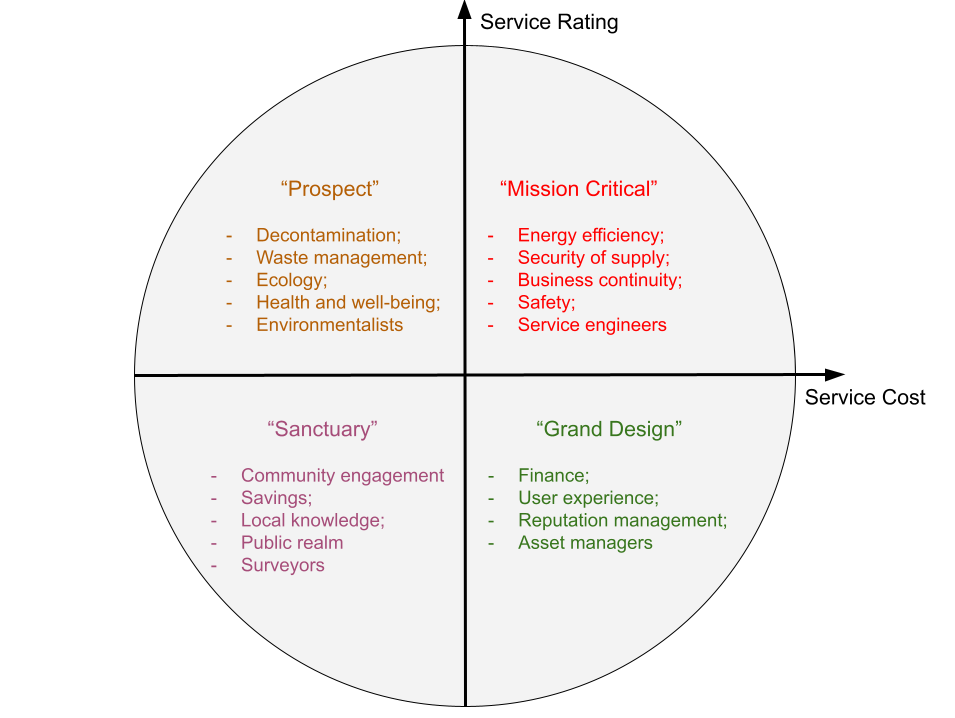
\includegraphics[width=1\textwidth]{scenarios}
\caption{Scenarios for Service Performance Marketing}
\label{Scenarios}
\end{figure}

\begin{table}[H]
\caption{Possible Site Typologies at Plausible Service Limits}
\begin{center}
\begin{tabular}{| l | l |}
\hline
Service Performance Scenario&Site Typology\\
\hline
Prospect&Landfill\\
Sanctuary&Tent\\
Mission Critical&Data Centre\\
Grand Design&Golf Club\\
\hline
\end{tabular}
\end{center}
\label{Service limits table}
\end{table}

Believing ones narrative to be reasonable, consideration is made towards selecting technologies for implementation.
Stable agreements of Ecosystem Performance and Service Rating may be made between any legal entities, including individuals and organisations.
Such agreements could be supported by distributed peer-to-peer blockchain, with peer endorsement of Ecosystem Performance and Service Rating transactions.
These transactions would be formed of standard contracts, defined in chaincode.
This could result in a fully auditable and assured enterprise grade root source of trust to enable secure transactions worldwide.\\

\section{Conclusions}

Restate the Thesis;
Summarize Key Points;
Provide Closure;
Leave a Lasting Impression

\begin{thebibliography}{99}

\bibitem{jr2} Rawls~J. (1999)
\emph{The Law of Peoples}
Cambridge, MA and London: Harvard University Press

\bibitem{jl1} Locke~J. (1967)
\emph{Two Treatises of Government}
Cambridge: Cambridge University Press
	
\bibitem{rn1} Nozick~R. (1974)
\emph{Anarchy, State and Utopia}
New York, NY: Basic Books
	
\bibitem{th1} Hobbes~T. (1668)
\emph{Leviathan},
Oxford: Oxford University Press

\bibitem{rc1} Coase~R.H. (1960)
\emph{The Problem of Social Cost.},
The Journal of Law and Economics, 3, pp. 1-44

\bibitem{pd3} Dasgupta~P. (2015)
\emph{Disregarded Capitals: What National Accounting Ignores.},
Accounting and Business Research, 45(4), pp. 122-138

\bibitem{hs1} Sidgwick~H. (1877)
\emph{The Methods of Ethics}
Cambridge: Cambridge University Press

\bibitem{pd2} Dasgupta~P. (2001)
\emph{Valuing Goods.},
In: Human Well-Being and the Natural Environment. Oxford: Oxford University Press, pp. 122-138

\bibitem{ka1} Arrow~K.J. (1963)
\emph{Social Choice and Individual Values},
New York, NY: John Wiley
	
\bibitem{km1} May~K. (1952)
\emph{A Set of Necessary and Sufficient Conditions for Simple Majority Decisions},
Econometrica, 20(4), pp. 680-684

\bibitem{as2} Sen~A. (1970)
\emph{Collective Choice and Social Welfare}
San Francisco: Hoden Day

\bibitem{jw2} Waldron~J. (1984)
\emph{Theories of Rights}
Oxford: Oxford University Press
		
\bibitem{rd1} Dworkin~R. (1978)
\emph{Taking Rights Seriously}
London: Duckworth

\bibitem{np1} The Nobel Prize (2021)
\emph{William D. Nordhaus, Facts},
Accessed 04/02/2021, available online: 
\url{https://www.nobelprize.org/prizes/economic-sciences/2018/nordhaus/facts/}

\bibitem{g1} Press Association (2007)
\emph{Peerage for climate change economist},
Accessed 04/02/2021, available online: 
\url{https://www.theguardian.com/environment/2007/oct/19/climatechange}

\bibitem{fr1} Ramsey~F.P. (1928)
\emph{A Mathematical Theory of Saving.}
Economic Journal, 38(152) pp. 543-559

\bibitem{wc1} Cline~W.R. (1992)
\emph{The Economics of Global Warming},
Washington D.C.: Institute for International Economics
		
\bibitem{wn1} Nordhaus~W.D. (1994)
\emph{Managing the Global Commons: The Economics of Climate Change},
Cambridge, MA: MIT Press
	
\bibitem{ns1} Stern~N.H. (2006)
\emph{The Stern Review of the Economics of Climate Change},
Cambridge: Cambridge University Press
		
\bibitem{ch1} Hope~C., Anderson~J., Wenman~P. (1993)
\emph{Policy Analysis of the Greenhouse Effect. An Application of the PAGE Model},
Energy Policy, 21, pp. 327-338
		
\bibitem{rsjt1} Tol~R.S.J. (1997)
\emph{On the Optimal Control of Carbon Dioxide Emissions: An Application of FUND},
Environmental Modelling and Assessment, 2, pp151-163

\bibitem{iwg1} Interagency Working Group on Social Cost of Carbon, United States Government (2013)
\emph{Technical Support Document: - Technical Update of the Social Cost of Carbon regulatory Impact Analysis - Under Executive Order 12866},
Washington D.C.: United States Government

\bibitem{jr1} Rawls~J. (1971)
\emph{A Theory of Justice}
Cambridge, MA and London: Harvard University Press

\bibitem{as1} Sen~A. (1961)
\emph{On Optimizing the Rate of Saving}
Economic Journal, 71
		
\bibitem{ms1} Marglin~S.A. (1961)
\emph{The Social Rate of Discount and The Optimal Rate of Investment}
The Quaterly Review of Economics, 77(1), pp. 95-111

\bibitem{fh1} Hayek~F. (1944)
\emph{The Road to Serfdom}
Chicago: University of Chicago Press

\bibitem{wbank} World Bank (2024)
\emph{World Development Indicators}
Accessed 13/11/2024, available online: 
\url{https://databank.worldbank.org/source/2?country=IRN&l=en}

\bibitem{imf} International Monetary Fund (2024)
\emph{IMF Data}
Accessed 13/11/2024, available online: 
\url{https://data.imf.org/en}

\bibitem{atp1} Parkinson~A.T., Friedman~K.S., Hacking T., Guthrie~P.M. (2012)
\emph{Exploring Scenarios for the Future of Energy Management in Property.},
Building Research and Information, 40(3), pp. 373-388
	
\end{thebibliography}



\end{document}